\documentclass[12pt]{extarticle}
\usepackage[default]{droidserif}
\usepackage[T1,T2A]{fontenc}
\usepackage[utf8]{inputenc}
\usepackage[bulgarian]{babel}
\usepackage{indentfirst}
\usepackage[a4paper, portrait, margin = 2cm]{geometry}
\usepackage{url}
\usepackage{color}
\usepackage{graphicx}
\usepackage{wrapfig}
\usepackage{csvsimple}
\usepackage{xcolor}
\renewcommand{\baselinestretch}{1.6}
\setlength{\emergencystretch}{3em}

\usepackage{color}
\definecolor{Bluish}{rgb}{0.39,0.55,0.78}

\newlength{\bulletwidth}\settowidth{\bulletwidth}{$\bullet$}
\newcommand{\mitem}{\vspace{5mm}\setlength{\leftskip}{\leftmargin}\hspace*{-\labelsep}\hspace*{-\bulletwidth}$\bullet$\hspace*{\labelsep}}
\newcommand{\mend}{\setlength{\leftskip}{0cm}\vspace{5mm}}


\usepackage{hyperref}
\hypersetup{
    colorlinks=true,
    linktoc=all,
    citecolor=black,
    filecolor=black,
    linkcolor=blue,
    urlcolor=blue
}

\title{t\textit{ray}tor - разпределен рейтрейсър}
\author{Диана Генева <dageneva@gmail.com> ФН 81008\\
Ангел Ангелов <hextwoa@gmail.com> ФН 81050}
\date{2016}

 
\begin{document}
\maketitle
\thispagestyle{empty}

\centerline{\url{https://github.com/DexterLB/traytor}}

\vspace{3cm}
\centerline{\includegraphics[width=\textwidth]{skull.png}}
\pagebreak

\section{Описание}
бла бла бла рейтрейсър бла бла (описание на проблемът, който решава
проектът)

\subsection{Задача}
Проектът ни имплементира рейтрейсър, който по дадена сцена генерира
картина. Симулира се светлината, както би се държала в реалната
(Нютонова) вселена, като се изстрелват лъчи от камерата, и се симулира
как те се удрят в обекти из сцената, докато стигнат до повърхност,
излъчваща светлина. Така получаваме пътя, изминат от един фотон до
камерата - и нещата, които се случват с този фотон, могат на практика да са само две:
\begin{itemize}
	\item Отражение
	\item Пречупване
\end{itemize}
Като при всяко едно такова събитие лъчът може да си промени цвета по
някакъв начин. Това е алгоритъмът \textbf{path tracing} - той е много
прост, но също така идеално възпроизвежда физиката:  всичко, което
можем да видим с очи, може да се репрезентира в сцена. Проблемът на
този алгоритъм е, че е \textbf{много, много, много бавен}. Макар че
можем да получим всичко само с тези два материала, се налага да имаме
например ''грапаво отражение'' (Ламбъртов материал), за да симулираме
твърди повърхности - иначе трябваше да моделираме всяка една грапавина
върху повърхността.

\pagebreak
\section{Архитектура}

Рейтрейсърът е реализиран на Go. Не са използвани други външни
библиотеки освен стандартната.

Потребителят има досег до следните части от проекта:

\mitem traytor render - команда за локално рендиране на сцена

\mitem traytor worker - работник, който се стартира на няколко машини

\mitem traytor client - клиент, който рендира разпределено на няколко
работници

\mitem Blender exporter - скрипт на Python, който създава сцена в
.json.gz формат, годна за прочитане от traytor

\mend

Рейтрейсърът поддържа текстури (включително HDR float), и те също
се пакетират чрез base64 кодиране във сценовия файл.

В тази документация ще разгледаме много накратко работата на самия
рейтрейсър, и ще обърнем повече внимание на паралелизацията. За
инструкции за ползване се обърнете към страницата на проекта 
(\url{https://github.com/DexterLB/traytor})
и \verb|traytor --help|, а за описание на имплементацията - към
техническата документация
(\url{https://godoc.org/github.com/DexterLB/traytor}).

\section{Имплементация}
Основният обект, който върши работа е \href{https://godoc.org/github.com/DexterLB/traytor/raytracer#Raytracer}{Raytracer}. Важната функция е \href{https://godoc.org/github.com/DexterLB/traytor/raytracer#Raytracer.Sample}{Sample()} - идеята е за всеки пиксел
от картинката да извикаме функцията \href{https://godoc.org/github.com/DexterLB/traytor/raytracer#Raytracer.Raytrace}{Raytrace()}.
Тя ще намери цвета, който ще има този лъч:


	\mitem Изстрелваме лъч от камерата, който отговаря на въпросните
	координати по екрана
	
	\mitem Гледаме къде (и дали) този лъч се пресича с триъгълната
	мрежа (\href{https://godoc.org/github.com/DexterLB/traytor/mesh#Mesh.Intersect}{Mesh.Intersect()}, като търсим триъгълника,
	който пресичаме в k-d дървото.
	
	\mitem Ако сме пресекли повърхност, знаем нейния материал.
	Извикваме \href{https://godoc.org/github.com/DexterLB/traytor/materials#Material}{Material.Shade()} за въпросната пресечна точка,
	и намираме получения цвят. Ако материалът е ''лампа'', това ще
	е дъното на рекурсията. Иначе материалът ще създаде нови лъчи
	и ще сметне цвета въз основа на техните цветове.

	\mend

Така получаваме картинка, която е много шумна. Сега трябва да повторим
същата операция много  пъти(100 е добро голямо число, a 1000: още по-добро \footnote{потвърдено от \href{https://www.fmi.uni-sofia.bg/bg/lecturers/ma/rnikolov}{ас. Росен Николов}}).

\subsection{Паралелизация по нишки (\href{https://github.com/DexterLB/traytor/blob/master/cmd/traytor/render.go}{traytor render})}

	\mitem стартират се n на брой нишки, като всяка
от тях инициализира свой \href{https://godoc.org/github.com/DexterLB/traytor/raytracer#Raytracer}{Raytracer} обект, със случайно генериран
random seed, и своя празна картинка

	\mitem Всяка от нишките намаля с 1 споделен брояч (\href{https://godoc.org/github.com/DexterLB/traytor/rpc#SampleCounter}{SampleCounter}) и добавя sample към картинката. Повтаря тази
	операция, докато броячът не е станал 0.
	
	\mitem В момента, която някоя от нишките стане готова (общият
	брояч е станал 0, и тя е свършила да рендира своя sample),
	изпраща картинката си по общ канал.
	
	\mitem Главната нишка събира всички изображения, получени по
	канала в едно, и накрая го записва като .png
	
	\mend
	
Така получаваме пълна паралелизация, и никоя от нишките не чака нищо
от друга преди последния момент, в който се събира резултатът.

\pagebreak
\subsection{Паралелизация по машини (\href{https://github.com/DexterLB/traytor/blob/master/cmd/traytor/worker.go}{traytor worker}, \href{https://github.com/DexterLB/traytor/blob/master/cmd/traytor/client.go}{traytor client})}
Тук имаме един клиент, комуникиращ чрез RPC библиотеката \href{https://godoc.org/github.com/valyala/gorpc}{gorpc} с много работници. Работниците слушат на някой TCP порт, а клиентът се 
свързва към тях, дава им работа и прибира резултата.

Имаме клас \href{https://godoc.org/github.com/DexterLB/traytor/rpc#RemoteRaytracerCaller}{RemoteRaytracerCaller} от страна на клиента, който вика функциите от \href{https://godoc.org/github.com/DexterLB/traytor/rpc#RemoteRaytracer}{RemoteRaytracer} от страна на
сървъра.


	\mitem Клиентът стартира лека нишка за всеки от работниците
	и извършва комуникацията с него в нея.

\begin{wrapfigure}{r}{7cm}
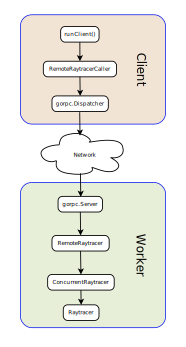
\includegraphics[width=7cm]{architecture.pdf}
\end{wrapfigure}
	
	\mitem Клиентът изпраща сцената на всеки от работниците
	(\href{https://godoc.org/github.com/DexterLB/traytor/rpc#RemoteRaytracer.LoadScene}{LoadScene()}). При получаване,
	работникат инициализира сцената (строи k-d дървото и т.н.)
	
	\mitem В момента, в който сме свършили да пращаме сцена на някой
	работник, стартираме толкова нишки за този клиент, колкото заявки
	може да получава (потребителски параметър max-requests) - добре е 
	да са повече, отколкото реалните нишки на работника, за да може
	да има ''изчакващи заявки'': така когато работникът свърши с
	рендирането на един sample, започва следващия без да чака
	резултатът от предния да се върне до клиента.
	
	\mitem Започваме цикъл, в който правим извиквания на \href{https://godoc.org/github.com/DexterLB/traytor/rpc#RemoteRaytracer.Sample}{Sample()}.
	Както при паралелизацията по нишки, имаме споделен брояч, който
	намаляваме, и по който разбираме кога да спрем да раздаваме
	работа на работниците.
	
	\mitem От страната на работника, имаме \href{https://godoc.org/github.com/DexterLB/traytor/rpc#ConcurrentRaytracer}{ConcurrentRaytracer},
	който съдържа буфер с толкова \href{https://godoc.org/github.com/DexterLB/traytor/raytracer#Raytracer}{Raytracer} обекти и съответните
	им картинки, колкото са нишките, които е поискал потребителя. Той
	се грижи винаги да се изпълняват не-повече от толкова
	\href{https://godoc.org/github.com/DexterLB/traytor/raytracer#Raytracer.Sample}{Sample()}
	функции едновременно, и всички едновременни извиквания да са
	върху различни \href{https://godoc.org/github.com/DexterLB/traytor/raytracer#Raytracer}{Raytracer} обекти, докато останалите
	заявки чакат в опашка. Това се реализира
	чрез буферираните канали в Go.
	
	\mitem Когато броячът стигне 0, и някой от работниците свърши
	със всичките си текущи заявки, клиентът извиква
	\href{https://godoc.org/github.com/DexterLB/traytor/rpc#RemoteRaytracerCaller.GetImage}{GetImage()}
	на този работник. От страната на работника отделните картинки
	се съединяват (те са толкова на брой, колкото са едновременните
	нишки), и като резултат се връща една картинка.
	
	\mitem При получаване на картинка от някой работник, клиентът я
	съединява с общата. Когато всички работници изпратят своя
	резултат, картинката се записва в .png

	\mend

\section{Тестови резултати}
Тестовите резултати са правени върху сравнително лека сцена (1116
точки, 2046 триъгълника). Сцената на заглавната страница има 12245
триъгълника и отне
41 минути и 21 секунди върху 15-те компютъра, използвани за тестове.
Моделът на череп е предоставен в Public Domain от Cole Harris.

Тестовата сцена след пакетирането има размер 250kb, а сцената с
черепа - 2.7mb.

\subsection{Паралелизация по нишки}
Тестовете са извършени върху \url{t5600.rmi.yaht.net}
(32 x Intel(R) Xeon(R) CPU E5-2660 0 @ 2.20GHz),
операционна система CentOS Linux 7.2.1511 чрез ZSH скрипт,
който за всеки брой нишки прави по 3 теста, и записва времената
в .csv файл.

\subsection{Паралелизация по машини}
Тестовете са извършени върху 15 машини в зала 314 на ФМИ,
всяка с по 4 ядра Intel(R) 2.8GHz, операционна система Windows 8.1
(workers) и клиент на Arch Linux, kernel 4.6.2

Главната пречка за ефективността беше мрежата в залата - почти
едновременно пращане на 10mb картинки от всички работници до клиента
се оказа доста натоварващо за суича.

Тестващият скрипт прави по 3 теста за всеки брой машини (1-15),
като на всеки тест избира n на брой произволни машини от всички.

\vspace{5mm}
Време за изпълнение ($T_n$):
\begin{center}
\includegraphics[width=\textwidth]{host_graphs/Tn.pdf}
\end{center}

Ускорение ($S_n = T_1 / T_n$):
\begin{center}
\includegraphics[width=\textwidth]{host_graphs/Sn.pdf}
\end{center}

Ефективност ($E_n = T_n / n$):
\begin{center}
\includegraphics[width=\textwidth]{host_graphs/Sn_n.pdf}
\end{center}

\subsection{Таблични данни по нишки}
бла
бла


\subsection{Таблични данни по машини}
\scriptsize
\begin{center}
\begin{tabular}{ | l l l | }
\hline
брой машини & време за изпълнение & машини (последен октет от IP адреса им) \\
\hline
1 & 522.592001792 & 129 \\
1 & 525.40900608 & 139 \\
1 & 519.013455104 & 136 \\
2 & 268.649498112 & 144,140 \\
2 & 272.02413824 & 145,142 \\
2 & 272.150567936 & 145,129 \\
3 & 186.231294976 & 137,141,146 \\
3 & 184.337114624 & 136,142,140 \\
3 & 179.980595456 & 143,134,140 \\
4 & 142.613297152 & 146,130,135,139 \\
4 & 141.431089664 & 136,145,135,139 \\
4 & 149.255761152 & 143,140,137,129 \\
5 & 118.692458496 & 144,130,137,129,146 \\
5 & 112.023823104 & 143,139,132,134,140 \\
5 & 113.827926528 & 140,132,143,129,136 \\
6 & 94.550666496 & 132,146,143,141,130,135 \\
6 & 108.538273792 & 134,129,143,135,141,142 \\
6 & 95.622235904 & 145,130,137,139,132,140 \\
7 & 387.322793472 & 146,142,136,143,135,144,140 \\
7 & 89.336597248 & 132,137,142,134,146,135,141 \\
7 & 91.65369472 & 132,136,145,139,143,141,130 \\
8 & 80.175658752 & 143,132,135,140,141,134,146,142 \\
8 & 78.349268736 & 142,132,130,134,143,135,145,140 \\
8 & 86.200088064 & 135,134,142,137,141,136,143,129 \\
9 & 76.654398464 & 143,137,129,140,141,136,139,134,146 \\
9 & 87.671195648 & 140,134,145,135,139,141,136,146,144 \\
9 & 75.471955456 & 135,134,146,141,142,139,129,136,137 \\
10 & 73.608510208 & 140,130,141,144,146,143,129,134,142,145 \\
10 & 70.692721664 & 146,140,143,142,135,134,130,129,144,139 \\
10 & 69.910379776 & 135,146,137,136,134,139,129,132,130,142 \\
11 & 55.195927552 & 144,130,132,146,136,142,137,139,145,134,140 \\
11 & 63.840565504 & 141,142,136,129,145,143,139,135,140,134,130 \\
11 & 56.68986624 & 144,143,146,145,141,134,129,130,139,140,135 \\
12 & 53.890988032 & 144,141,130,129,139,137,143,146,135,140,142,136 \\
12 & 58.921648128 & 129,143,144,141,134,130,146,137,132,136,139,140 \\
12 & 58.510476032 & 146,137,136,139,145,140,132,135,130,134,142,129 \\
13 & 52.009936384 & 134,139,145,141,146,135,144,143,137,130,140,132,129 \\
13 & 53.823009536 & 136,129,144,141,135,142,132,145,134,143,146,139,130 \\
13 & 55.163354624 & 137,145,129,139,130,136,142,143,144,146,140,134,141 \\
14 & 49.592190464 & 136,134,139,130,142,141,146,143,140,145,129,135,132,144 \\
14 & 49.900462592 & 142,144,146,143,140,135,132,134,137,136,130,145,129,141 \\
14 & 54.727507968 & 139,140,132,134,141,137,146,129,142,144,143,135,145,136 \\
15 & 52.844302592 & 130,134,132,129,144,137,140,145,141,139,136,143,135,146,142 \\
15 & 49.135457024 & 144,146,136,134,129,139,140,143,142,132,137,135,141,145,130 \\
15 & 52.671005184 & 139,142,146,130,129,132,144,136,145,135,143,141,137,134,140 \\
\hline
\end{tabular}
\end{center}
\end{document}

